\section{Claude Mythos}
\label{sec:claude-mythos}

Mit der Veröffentlichung von Claude Mythos hat Anthropic im April 2026
ein LLM vorgestellt, welches fortgeschrittene Fähigkeiten im Cyberbereich aufweist \cite{anthropic_mythos_preview, aisi_claude_mythos_2026}.
Im Unterschied zu bisherigen Sprachmodellen, die offensive
Sicherheitsanalysen in der Regel als assistierende Werkzeuge unterstützen,
ist Mythos in der Lage, den gesamten Prozess der Schwachstellenforschung --
von der initialen Erkennung über die Exploit-Entwicklung bis zur
mehrstufigen Angriffskette -- ohne menschliches Eingreifen durchzuführen.
Claude Mythos war bereits in der Lage, Zero-Day-Schwachstellen in weit
verbreiteten Betriebssystemen und Webbrowsern zu identifizieren sowie
funktionsfähige Exploits zu generieren \cite{anthropic_mythos_preview}.
Dabei beschränkt sich das Modell nicht auf bekannte Schwachstellenklassen;
es ist darüber hinaus in der Lage, mehrere Schwachstellen miteinander zu
verknüpfen und so mehrstufige Angriffsketten zu konstruieren, die einzelne
Lücken erst in Kombination ausnutzbar machen \cite{anthropic_mythos_preview}.

Besondere Bedeutung kommt der Fähigkeit zu, auch sehr alte, bislang
übersehene Schwachstellen aufzudecken. Ein dokumentiertes Beispiel stellt
die autonome Ausnutzung einer 17~Jahre alten Schwachstelle dar, die zu
einer Remote Code Execution in FreeBSD führte und Root-Rechte
auf einem mit NFS verbundenen Server ermöglichte
(CVE-2026-4747) \cite{anthropic_mythos_preview}. Entscheidend ist dabei,
dass Mythos diesen Prozess vollständig autonom durchführte -- die
einzige menschliche Interaktion bestand in der ursprünglichen Aufforderung
zu Beginn der Sitzung. Im Vergleich dazu erforderte Claude Opus~4.6 für
äquivalente Aufgaben durchgehend menschliche Anleitung und war nicht in der
Lage, derartige Exploit-Ketten eigenständig zu schließen
\cite{anthropic_mythos_preview}.

Ein weiterer sicherheitsrelevanter Aspekt liegt in der Zugänglichkeit
des Modells: Da Mythos keine Vorerfahrung im Bereich der Penetrationstests
oder der Exploit-Entwicklung voraussetzt, können auch technisch nicht
versierte Nutzerinnen und Nutzer komplexe Angriffe initiieren
\cite{anthropic_mythos_preview, aisi_claude_mythos_2026}. Dies senkt die
Einstiegshürde für offensive Cyberaktivitäten erheblich und stellt
eine qualitativ neue Bedrohungsdimension dar.

Hervorzuheben ist, dass Mythos nicht explizit auf diese offensiven
Cyberfähigkeiten trainiert wurde; sie resultieren vielmehr als Nebenprodukt allgemeiner Verbesserungen in den Bereichen Code, Reasoning
und Autonomie \cite{anthropic_mythos_preview}. Dieselben Fähigkeiten, die das
Modell beim Schließen von Sicherheitslücken wirksamer machen, steigern
gleichermaßen seine Effektivität bei deren Ausnutzung -- was die Doppelnatur des Modells als defensives wie offensives Werkzeug
grundlegend unterstreicht \cite{anthropic_glasswing}.

Um die defensiven Potenziale gezielt nutzbar zu machen, initiierte
Anthropic im Frühjahr 2026 das \emph{Project Glasswing}: eine kontrollierte
Zugangsumgebung, die einer begrenzten Gruppe und Anbieter kritischer Softwareinfrastruktur Zugang zu Mythos-Fähigkeiten
gewährt \cite{anthropic_glasswing}. Ziel ist es, Schwachstellen in
kritischer Open-Source-Software systematisch zu identifizieren und durch
koordinierte Offenlegung (\emph{Coordinated Vulnerability Disclosure},
CVD) zu beheben \cite{anthropic_cvd}.

Im Rahmen dieses Programms hat Claude Mythos Preview seit Februar 2026
insgesamt 23.019~Schwachstellenkandidaten in Open-Source-Projekten
identifiziert \cite{anthropic_cvd_dashboard}. Nach Triage durch sechs
externe Sicherheitsforschungsunternehmen konnten 1.726~Funde als valide
Schwachstellen bestätigt werden (True-Positive-Rate: 90,8~\%), von
denen 1.596 gegenüber den jeweiligen Maintainern offengelegt wurden
\cite{anthropic_cvd_dashboard}. Stand 22.~Mai~2026 wurden dabei
281~Open-Source-Projekte untersucht und 88~CVE-Einträge
(\emph{Common Vulnerabilities and Exposures}) bzw.\
GHSA-Advisories (\emph{GitHub Security Advisory}) publiziert.
Abbildung~\ref{fig:cvd-dashboard} veranschaulicht den mehrstufigen
Prozess vom Aufdecken der Schwachstelle bis zur gepatchten Schwachstelle.

\begin{figure}[ht]
	\centering
	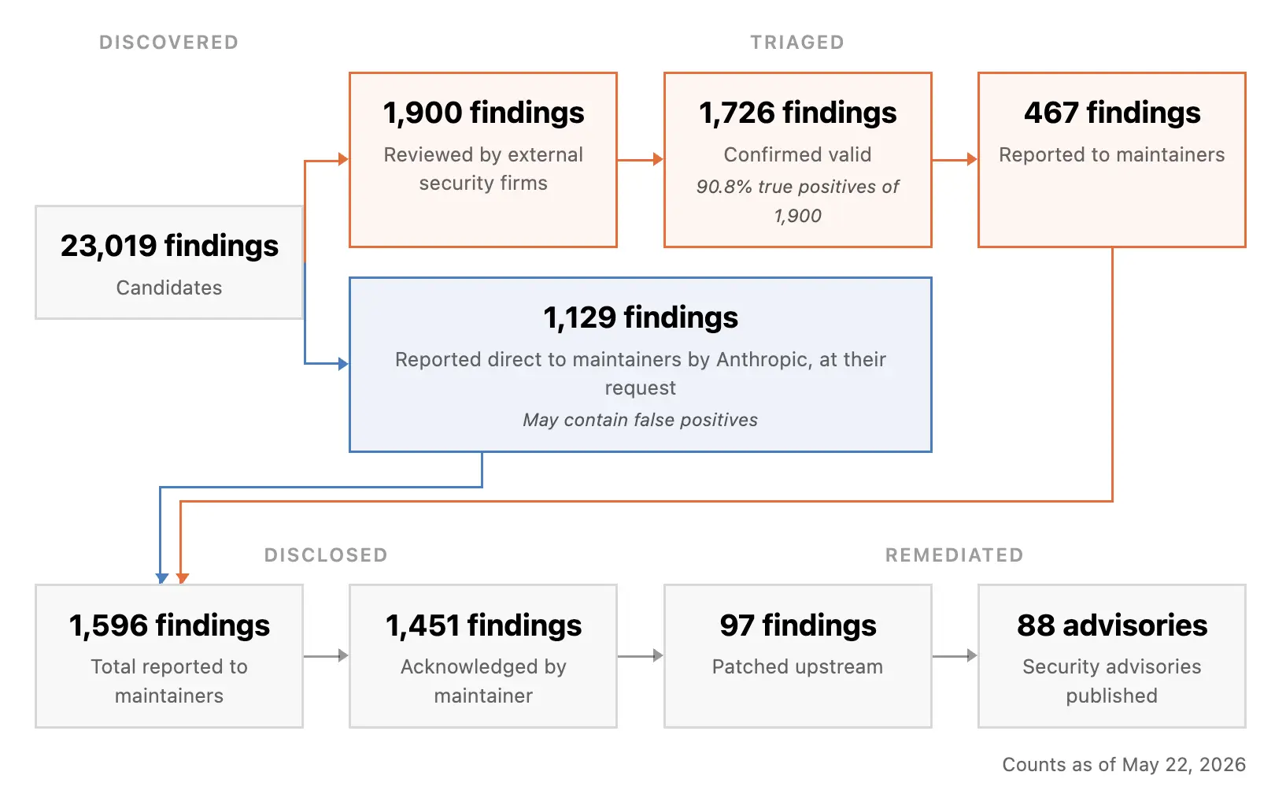
\includegraphics[width=\columnwidth]{images/mythos_disclosed.png}
	\caption{Coordinated Vulnerability Disclosure Dashboard von Anthropic
		(Stand: 22.~Mai~2026). Quelle: \cite{anthropic_cvd_dashboard}.}
	\label{fig:cvd-dashboard}
\end{figure}

Trotz dieser Fortschritte ist ein erheblicher Anteil der identifizierten
Schwachstellen bislang ungepatcht: Von den 1.596~offengelegten Funden
wurden lediglich 97~upstream behoben, was einer Patch-Rate von rund
6~\% entspricht \cite{anthropic_cvd_dashboard}. Dies ist einerseits
auf die begrenzte Kapazität der Maintainer zurückzuführen; andererseits
stellt die Geschwindigkeit, mit der Mythos neue Schwachstellen produziert,
die klassischen CVD-Prozesse vor erhebliche Skalierungsprobleme.

Im Juni 2026 veröffentlichte Anthropic mit \emph{Claude Fable 5} ein
weiteres Modell der Mythos-Klasse, das für den öffentlichen Einsatz
konzipiert wurde \cite{anthropic_fable5_mythos5}. Der Name leitet sich
vom lateinischen \emph{fabula} ab und ist bewusst als Pendant zu
\emph{Mythos} gewählt worden: Der einzige funktionale Unterschied
zwischen beiden Modellen besteht in einem neuartigen Klassifikator-System,
das bei Fable~5 sicherheitskritische Anfragen -- insbesondere aus den
Bereichen Cybersicherheit, Biologie und Chemie --
abfängt und an das schwächere Modell Claude Opus~4.8 weiterleitet
\cite{anthropic_fable5_mythos5}. Interne Messungen zeigen, dass dieser
Fallback in mehr als 95~\% aller Sitzungen nicht ausgelöst wird; für
die übrigen Sitzungen entspricht die Leistung von Fable~5 damit
nahezu derjenigen von Mythos~5 \cite{anthropic_fable5_mythos5}.
Claude Mythos~5 -- die identische Modellbasis ohne die genannten
Schutzmaßnahmen -- bleibt ausschließlich verifizierten Partnern im
Rahmen von Project Glasswing vorbehalten und soll sukzessive über
ein formalisiertes Trusted-Access-Programm in Konsultation mit der
US-Regierung erweitert werden \cite{anthropic_fable5_mythos5}.

Bereits drei Tage nach dem Launch, am 12.~Juni~2026, sah sich Anthropic
gezwungen, den Zugang zu Fable~5 und Mythos~5 für alle Nutzer weltweit
zu sperren \cite{anthropic_fable5_access}. Auslöser war eine behördliche
Exportkontrollanweisung der US-Regierung, die unter Berufung auf
nationale Sicherheitsinteressen den Zugang für alle ausländischen
Staatsangehörigen -- auch innerhalb der Vereinigten Staaten -- untersagte
\cite{anthropic_fable5_access}. Da Anthropic keine Möglichkeit hatte,
die Staatsbürgerschaft von Nutzern in Echtzeit zu verifizieren, wurde
der Zugang zu beiden Modellen vollständig eingestellt. Hintergrund war
ein von Amazon-Forschern entdecktes Verfahren zur Umgehung der
Sicherheitsklassifikatoren von Fable~5, bei dem das Modell durch
gezielte Prompts dazu gebracht werden konnte, Softwareschwachstellen
zu identifizieren und in einem Fall Code zur Demonstration eines
Exploits zu produzieren \cite{anthropic_redeploying_fable5}.
Anthropic widersprach der behördlichen Einschätzung öffentlich: Eigene
Tests hätten gezeigt, dass schwächere Modelle -- darunter Claude
Opus~4.8, GPT-5.5 und Kimi~K2.7 -- dieselben Schwachstellen identifizieren
konnten, ohne dass eine Umgehung der Schutzmaßnahmen notwendig gewesen
wäre \cite{anthropic_redeploying_fable5}. Der gefundene Jailbreak ermögliche damit keinen Zugriff auf die
einzigartigen Fähigkeiten von Mythos, sondern betreffe lediglich
gewöhnliche Aufgaben der defensiven Cybersicherheit
\cite{anthropic_fable5_access, anthropic_redeploying_fable5}.

Nachdem Anthropic in enger Abstimmung mit der US-Regierung einen
verbesserten Sicherheitsklassifikator entwickelt hatte, der die
beschriebene Umgehungstechnik in über 99~\% der Fälle blockiert,
wurden die Exportkontrollen am 30.~Juni~2026 aufgehoben
\cite{anthropic_redeploying_fable5}. Ab dem 1.~Juli~2026 war Fable~5
weltweit wieder verfügbar. Im Zuge des Redeployments veröffentlichten
Anthropic, Amazon, Microsoft, Google und weitere Glasswing-Partner
einen gemeinsamen Entwurf für ein industrieweites Framework zur
einheitlichen Bewertung der Schwere von KI-Jailbreaks, das vier
Kriterien umfasst: den erzielten Fähigkeitsgewinn (\emph{capability gain}),
die Breite des Fähigkeitsgewinns, den Aufwand zur Weaponisierung sowie
die Auffindbarkeit der Technik \cite{anthropic_redeploying_fable5}.
Ziel ist es, neue Jailbreak-Funde künftig einheitlich bewerten und
behördliche Reaktionen daran ausrichten zu können.